\chapter{Design}\label{ch:design}

\section{High Level Design}\label{sec:ch4-hld}

The work falls into two halves, and the only thing they share is the trained detector checkpoint. The \emph{offline} half is where the models are developed. Public datasets are converted to a single pothole class, near-duplicate images are grouped, and the data is split so that no group ends up in two splits; YOLOv8s detectors are then trained and evaluated under a fixed protocol. The \emph{online} half is the application. A user uploads phone or dashcam video together with its GPS log, and the system finds the potholes, follows each one from frame to frame and attaches the camera position. It then merges repeated sightings into mapped potholes, places them on an OpenStreetMap road graph, computes statistics for each road segment and plans routes that take potholes into account. All of this is available through a REST API and a browser interface.

A few design decisions, written down at the start, shaped the rest of the system:
\begin{itemize}[itemsep=0pt]
\item Potholes are detected as boxes of a single class. Segmentation and severity grading were left out of scope.
\item Raw records (sessions, GPS fixes, jobs and observations) are stored separately from anything derived from them, such as mapped potholes, surveyed road and segment statistics. The derived tables are rebuilt from scratch after each successful job.
\item No data is discarded without a record. Excluded images and rejected GPS rows are logged with the reason, and when the geotagging function cannot place an observation it returns no position instead of guessing one.
\item A road that nobody has surveyed is never counted as pothole-free, and synthetic demonstration data is kept apart from real recordings.
\item Every threshold in the pipeline is provisional, and none of them was tuned on test data.
\end{itemize}

For each road segment, meaning an undirected edge of the OpenStreetMap graph, the system stores how many mapped potholes lie on it, how much of it has been surveyed, and the resulting rate per 100 m. Each route is also given the share of its length that was surveyed and an evidence level. No severity, score or grade is computed.

\section{System Architecture}\label{sec:ch4-arch}

As Figure~\ref{fig:ch4-architecture} shows, the whole application runs inside a single server process. FastAPI serves the REST API under \texttt{/api} and the web pages from \texttt{/}. Uploaded sessions wait in an in-memory queue until the job runner, a single worker thread, picks them up one by one. The data is kept in SQLite with write-ahead logging, while uploaded videos and annotated detection images sit in folders next to the database file. Because the road graph is a JSON file produced once by an offline OSMnx download \cite{boeing2017osmnx}, routing needs no network connection. Only the background map tiles are fetched from the internet.

\begin{figure}[!htbp]
\centering
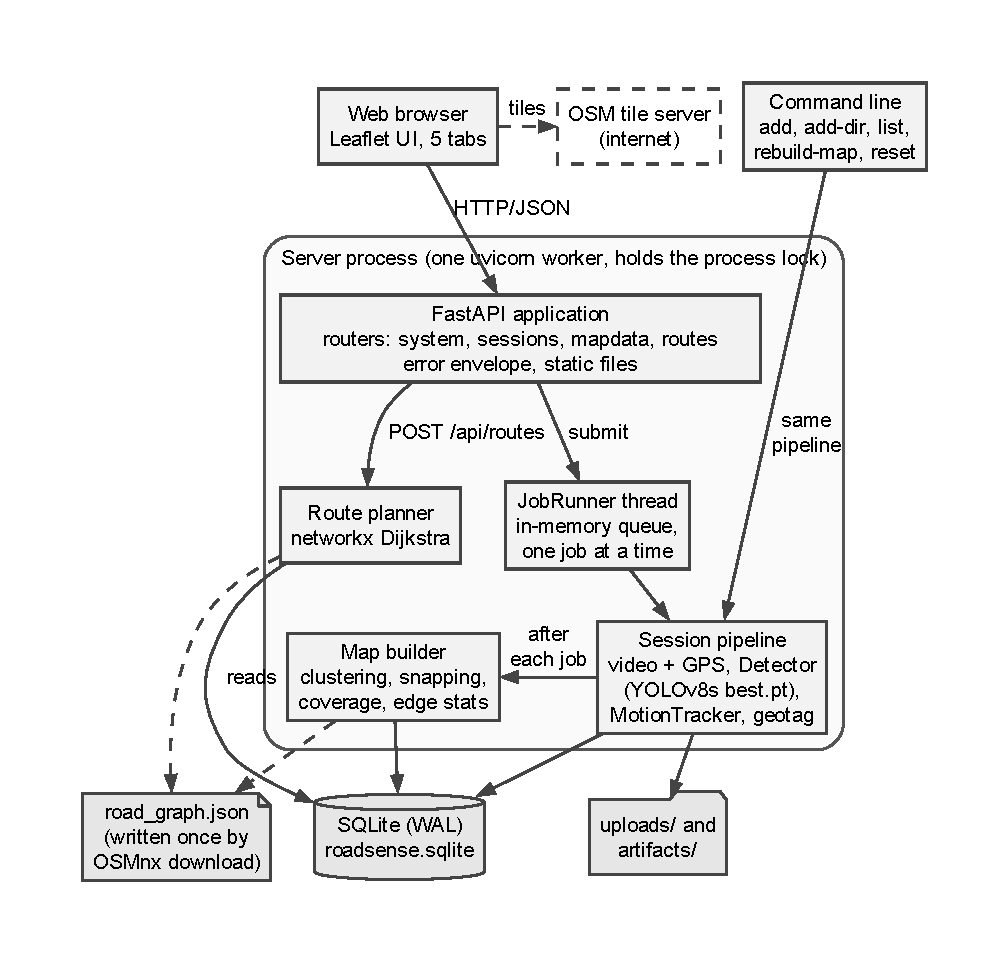
\includegraphics[width=0.68\textwidth]{ch4_architecture.pdf}
\caption{Runtime architecture. Solid arrows are calls or data flow; dashed arrows are read-only access or the optional base map.}
\label{fig:ch4-architecture}
\end{figure}

When it starts, the application uses the operating system to lock a file beside the database. A second server, or a command-line process that writes data, therefore cannot use the same database at the same time. Since no other process can own a job, any job still marked queued or running from an earlier run can safely be set to failed. A job whose detector fails on 2\% of the analysed frames or fewer is complete; up to 25\% it is kept as partial with a warning, and beyond that it fails and nothing is stored. Figure~\ref{fig:ch4-dataflow} traces a single recording from upload through to the map.

\begin{figure}[!htbp]
\centering
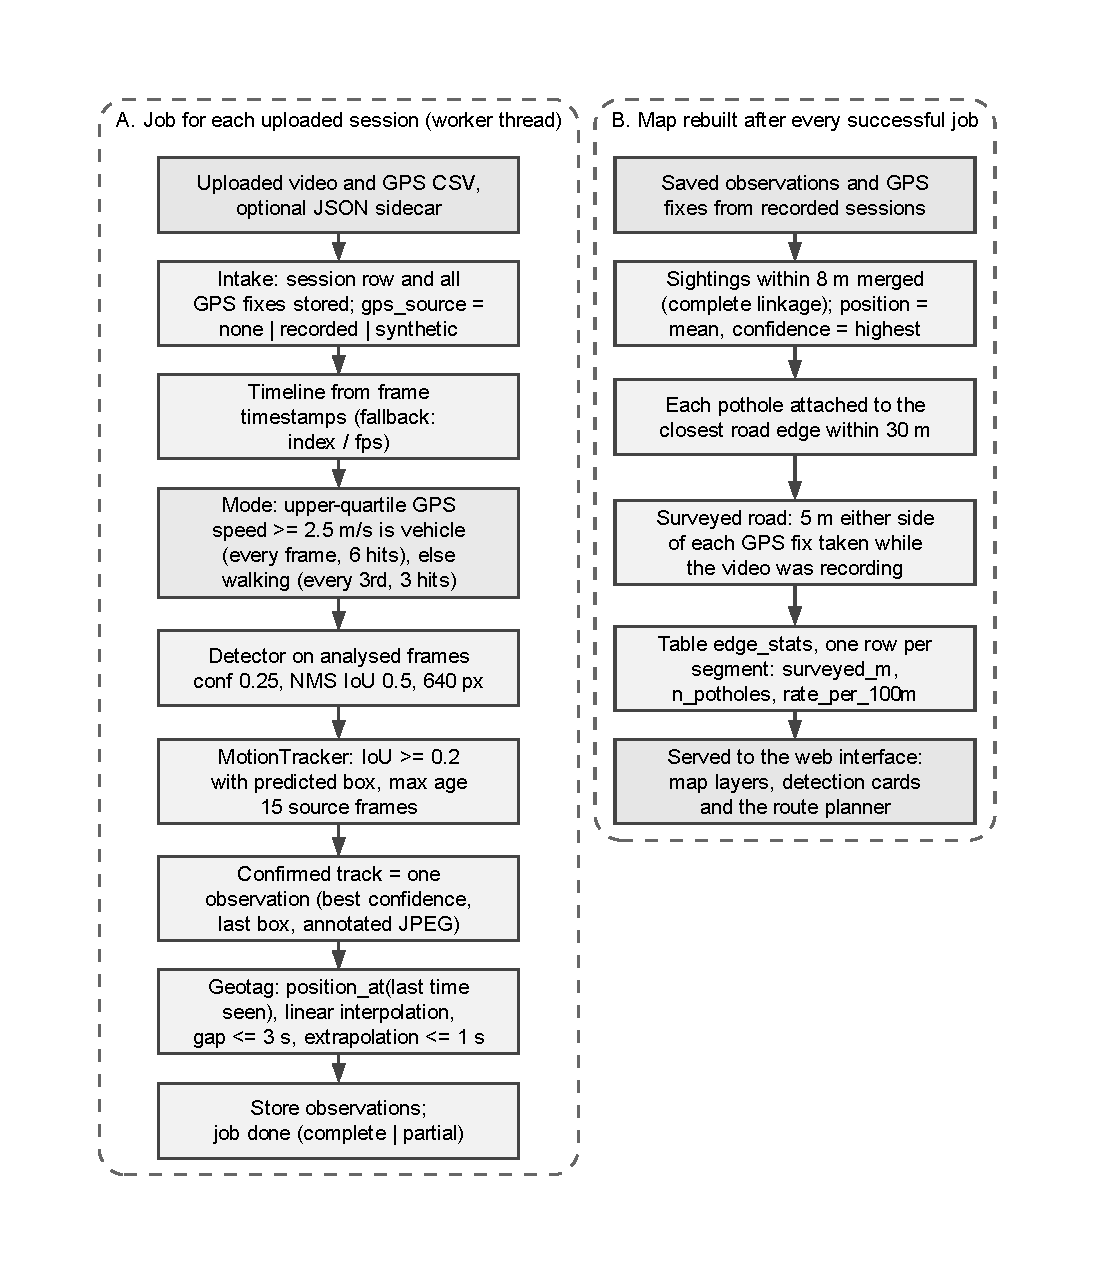
\includegraphics[width=0.62\textwidth]{ch4_dataflow.pdf}
\caption{How an uploaded video and GPS log become mapped potholes and road-segment statistics. Part A is the job run for each session and part B the map rebuild; the parameter values shown are the application defaults.}
\label{fig:ch4-dataflow}
\end{figure}

\subsection{Database structure}\label{sec:ch4-db}
All data lives in one SQLite file. It uses write-ahead logging and enforced foreign keys, and its schema carries a version number, currently 2, with no migration scripts between versions. Figure~\ref{fig:ch4-er} shows its nine tables. Four hold raw data: \texttt{sessions}, \texttt{gps\_fixes}, \texttt{jobs} and \texttt{observations} (one confirmed track with its best confidence, box, image and camera position). Four hold derived data that every map build wipes and recomputes: \texttt{builds}, \texttt{potholes}, \texttt{edge\_coverage} and \texttt{edge\_stats}. The table \texttt{meta} holds settings. A road segment is identified by its two OpenStreetMap node identifiers and edge key; because these are only meaningful for one graph, each build records the graph hash and routing refuses a build made with another graph.

\begin{figure}[!htbp]
\centering
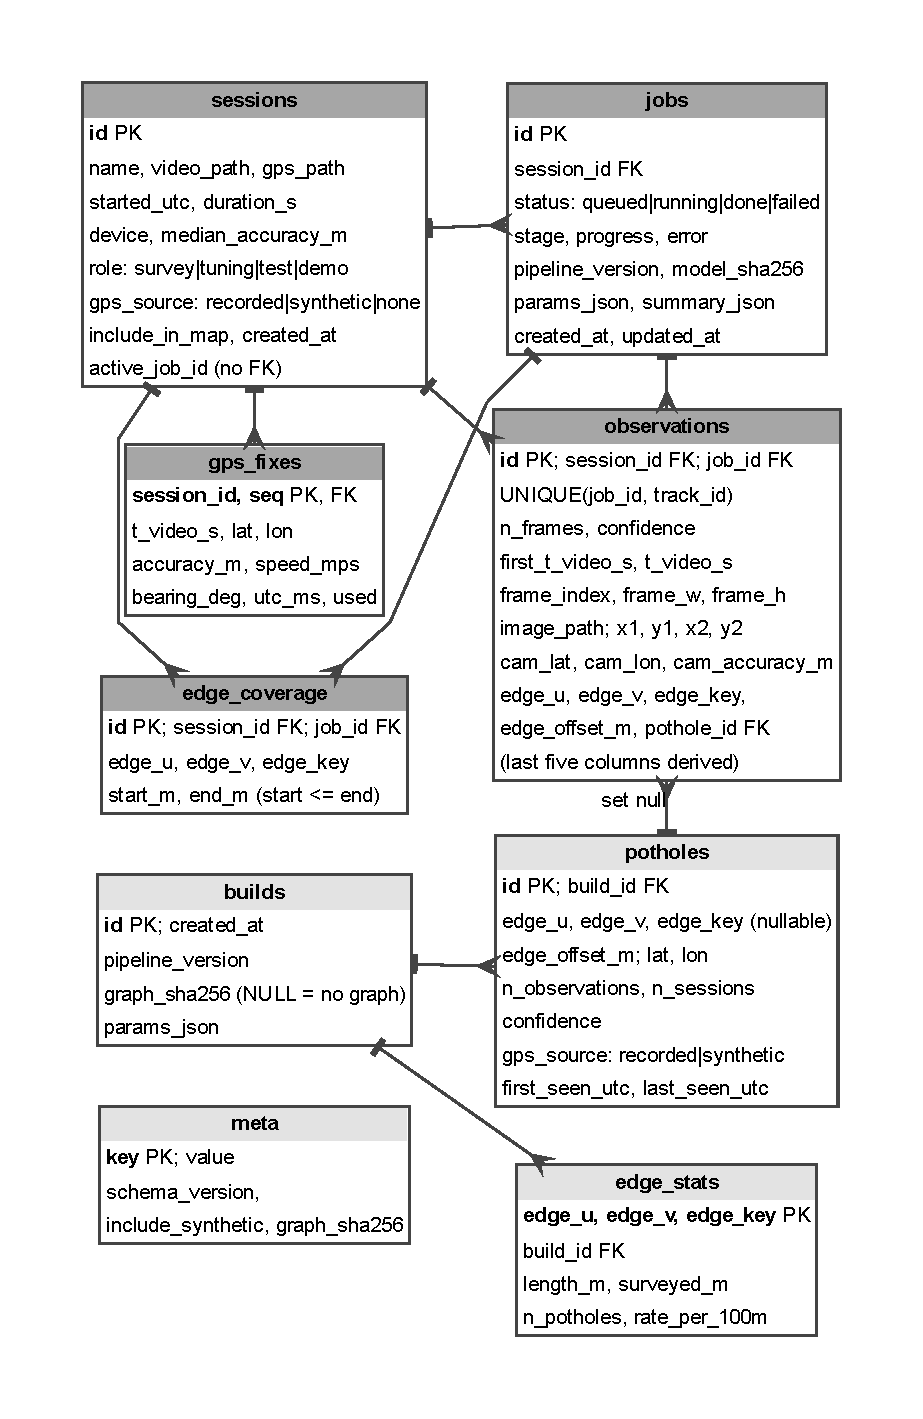
\includegraphics[width=0.55\textwidth]{ch4_er.pdf}
\caption{Entity-relationship diagram. Dark headers are raw tables; light headers are derived and control tables.}
\label{fig:ch4-er}
\end{figure}

\section{Use-case Diagram}\label{sec:ch4-usecase}
The system has no user accounts. Figure~\ref{fig:ch4-usecase} shows three actors: the user of the web interface, any other HTTP client (which can perform the same operations, since the interface calls only documented endpoints), and a person at the machine who uses the command line to add recordings, list sessions, rebuild the map or reset the database.

\begin{figure}[!htbp]
\centering
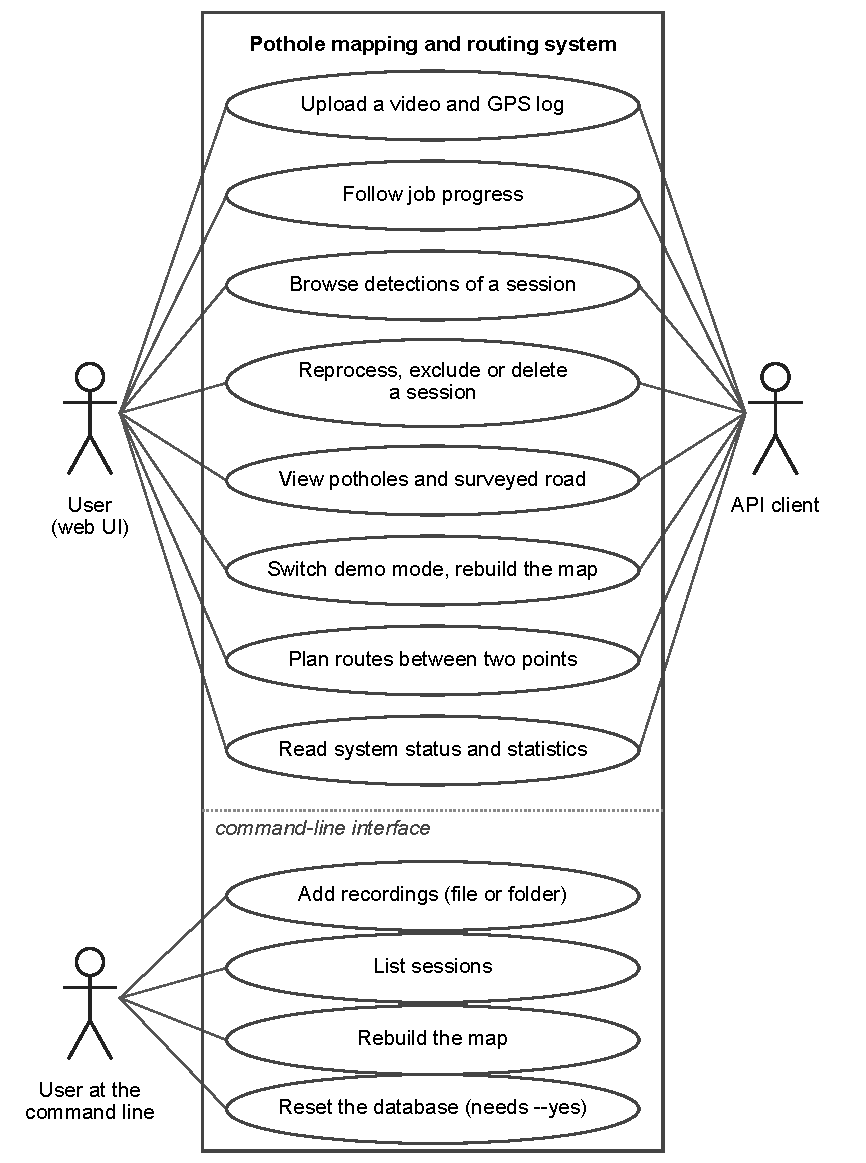
\includegraphics[width=0.58\textwidth]{ch4_usecase.pdf}
\caption{Use-case diagram. The web interface is itself a client of the API.}
\label{fig:ch4-usecase}
\end{figure}

\section{Class Diagram}\label{sec:ch4-class}
Most of the code consists of plain functions and small data classes rather than deep class hierarchies. Figure~\ref{fig:ch4-class-pipeline} covers the detection pipeline. For each job, the runner calls \texttt{process\_session}, which picks a tracking plan, runs the detector over the sampled frames and hands the detections to a \texttt{MotionTracker}. The pipeline talks to the detector only through the \texttt{DetectorLike} protocol. In normal use the \texttt{Detector} class fulfils it with an Ultralytics model, while the tests plug in a fake detector instead. On the service side, \texttt{EdgeIndex} snaps points onto road edges, and both the map builder and \texttt{plan\_routes} are functions that read the road graph and the database.

\begin{figure}[!htbp]
\centering
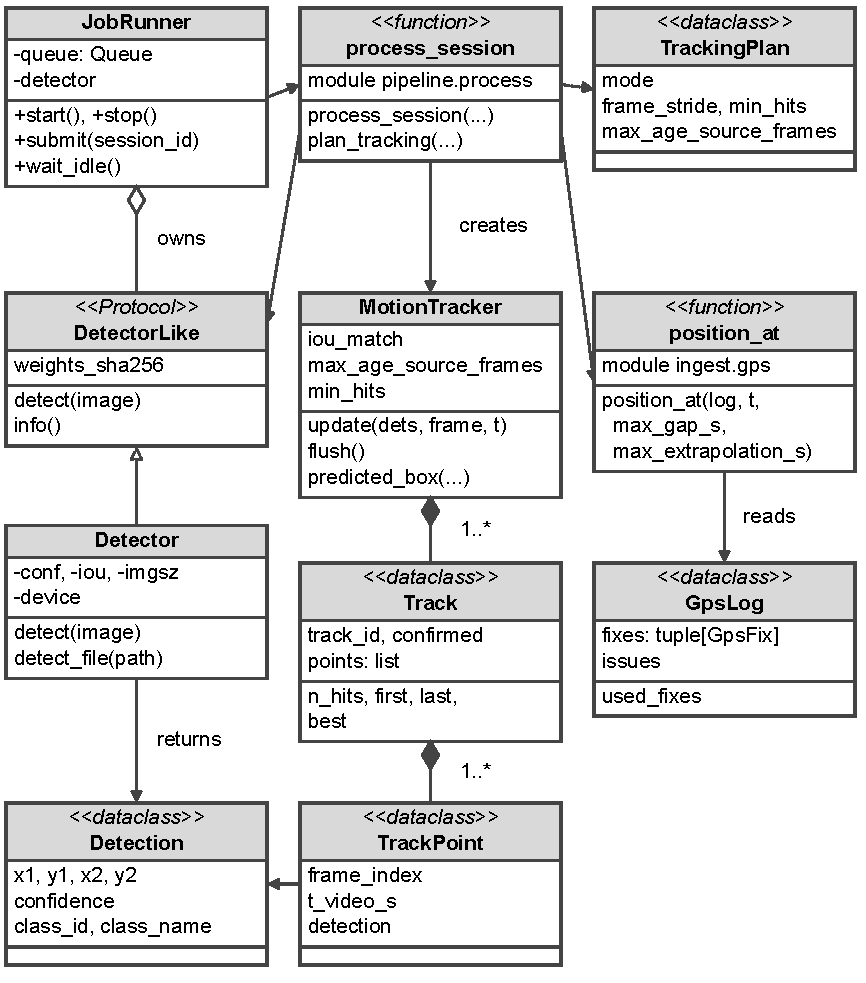
\includegraphics[width=0.66\textwidth]{ch4_class_pipeline.pdf}
\caption{Classes and function modules of the detection pipeline.}
\label{fig:ch4-class-pipeline}
\end{figure}

\section{Sequence Diagram}\label{sec:ch4-seq}
Figure~\ref{fig:ch4-seq-upload} follows an upload. Before replying with status 202, the API has already saved the session and its GPS fixes and created the job, so detection never happens inside the request itself. From then on the browser asks for the job status once a second. Meanwhile the worker runs the pipeline, saves the observations and the job status in a single transaction, and rebuilds the map. A route request, by contrast, is answered straight away from the stored map.

\begin{figure}[!htbp]
\centering
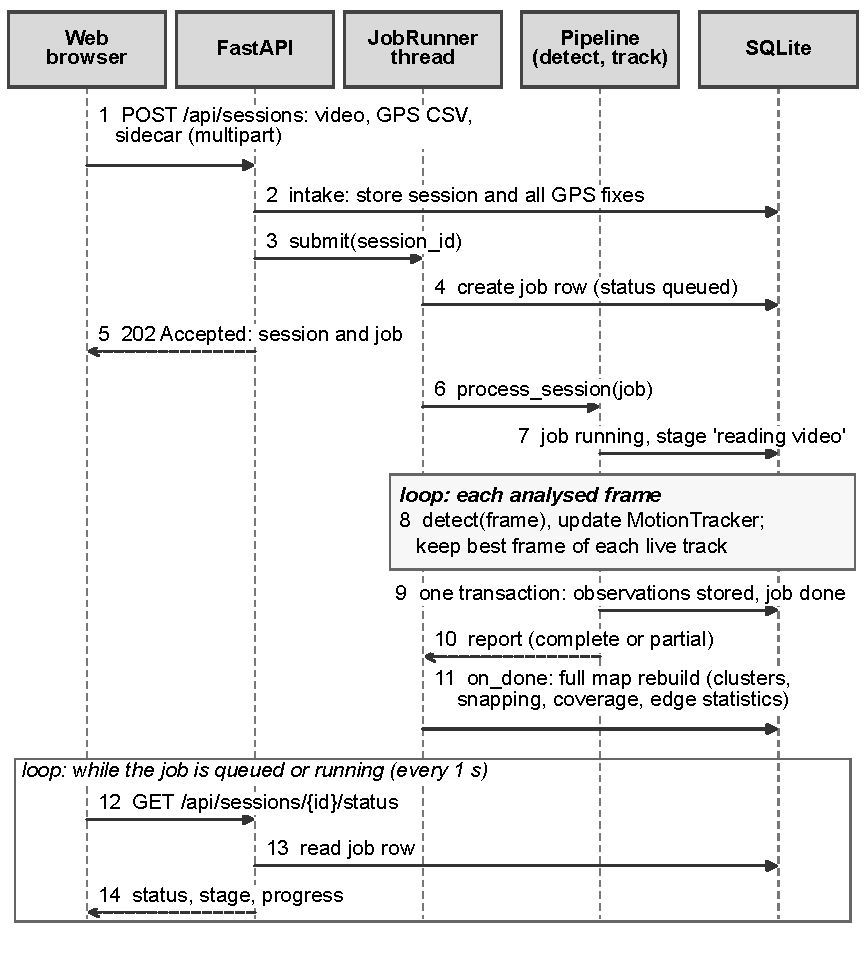
\includegraphics[width=0.72\textwidth]{ch4_seq_upload.pdf}
\caption{Sequence diagram for uploading and processing a session.}
\label{fig:ch4-seq-upload}
\end{figure}

\section{Detection-to-Map Pipeline Design}\label{sec:ch4-pipeline}

\subsubsection*{Sampling mode}
The upper quartile of the GPS speeds in the session decides the mode. At 2.5 m/s or more the session is a vehicle recording: every frame is analysed and a track needs 6 detections to be confirmed. Otherwise every third frame is analysed and 3 detections suffice. The upper quartile is used so that a ride with long stops is still treated as a vehicle recording.

\subsubsection*{Motion-aware tracker}
At vehicle speed a pothole can move further between analysed frames than its own height, so its boxes in consecutive frames may not overlap. The tracker therefore predicts each live track's box by shifting its last box by the track's average centre velocity over up to its last six points, and matches detections to predicted boxes greedily by intersection over union (IoU) of at least 0.2. A track ends after 15 source frames without a match; a track with enough hits becomes one observation. It is a simple tracker with no Kalman filter or appearance model, chosen over ByteTrack \cite{zhang2022bytetrack} to avoid an extra dependency.

\subsubsection*{Geotagging}
An observation is positioned at the camera location at the time $t$ the track was last seen, by linear interpolation between the bracketing GPS fixes at times $t_a \le t \le t_b$ with positions $p_a$ and $p_b$:
\begin{equation}
p(t)=p_a+\frac{t-t_a}{t_b-t_a}\,(p_b-p_a).
\label{eq:ch4-interp}
\end{equation}
No position is returned if the fixes are more than 3 s apart, and fixes with accuracy worse than 25 m are not used. No forward offset is applied, so a mapped pothole lies a few metres behind its true position, plus GPS error.

\subsubsection*{De-duplication and snapping}
Sightings from several tracks or passes are merged by greedy complete linkage: a set of sightings forms one mapped pothole only if every pair is within 8 m. Complete linkage replaced single linkage, which chained a line of sightings into one long pothole. Each mapped pothole is then snapped to the nearest road edge within 30 m; snapping is per point, so it can choose the wrong one of two close parallel roads.

\subsubsection*{Surveyed length}
A segment counts as surveyed only where a recorded session's GPS trace, clipped to the video interval, actually ran: each fix covers 5 m on either side, and consecutive fixes at most 3 s apart fill the span between them. For each edge the builder stores the surveyed length $s$, the number of mapped potholes $n$ and the rate $100\,n/s$ potholes per 100 m.

\section{Route-cost Design}\label{sec:ch4-route}
Road that has not been surveyed is unknown, not clean. For a directed edge of length $L$ metres with $n$ mapped potholes and $s$ surveyed metres, the router estimates the expected potholes as
\begin{equation}
E=n+r\,\frac{L-s}{100},
\qquad
r=\frac{100\,N+r_0\,\psi}{S+\psi},
\label{eq:ch4-expected}
\end{equation}
where $r$ is the assumed rate per 100 m on unsurveyed road, $N$ and $S$ are the mapped on-road potholes and surveyed metres over the whole map, and $r_0=1.0$ per 100 m and $\psi=500$ m are stated assumptions. The rate starts at $r_0$ and moves toward the observed rate as more road is surveyed, so one pothole on a few metres cannot produce an extreme value. The cost of the edge for an avoidance setting $a\in[0,1]$ is
\begin{equation}
\mathrm{cost}=L+a\,\lambda\,E,\qquad \lambda=300\ \mathrm{m},
\label{eq:ch4-cost}
\end{equation}
so at $a=1$ the router accepts a 300 m detour to avoid one expected pothole. The cost has no severity, confidence weighting or traffic term.

The router runs Dijkstra's algorithm \cite{dijkstra1959note} three times, for $a=0$ (Shortest), the user's setting, and $a=1$ (Strongest pothole avoidance), and merges identical routes, so it returns one to three routes. For each it reports the distance, a travel time from speed limits, the mapped potholes passed, the surveyed share $f$ of its length, and an evidence level: adequate if $f\ge0.8$, partial if $0.2\le f<0.8$ and insufficient otherwise. These thresholds, like $r_0$, $\psi$ and $\lambda$, are configuration values that have not been validated. Generated text never calls a road safe, clear or pothole-free. Figure~\ref{fig:ch4-routecost} shows the computation.

\begin{figure}[!htbp]
\centering
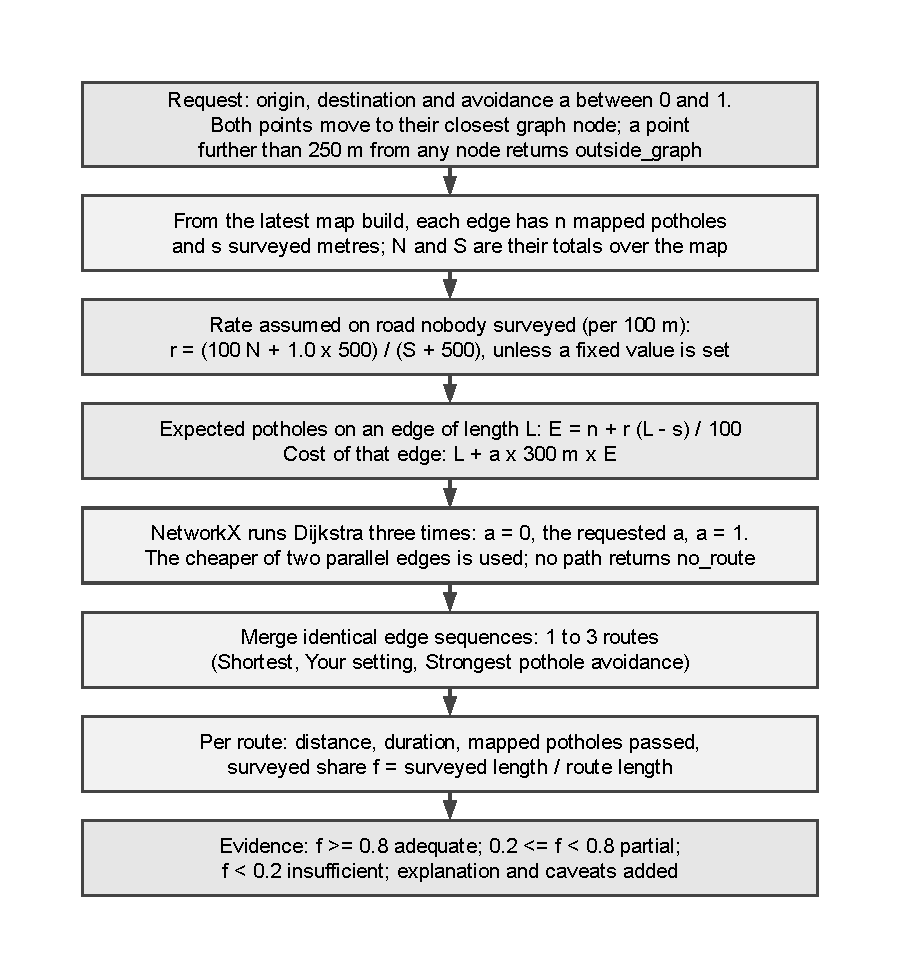
\includegraphics[width=0.5\textwidth]{ch4_routecost.pdf}
\caption{Route-cost computation from a request to a route plan.}
\label{fig:ch4-routecost}
\end{figure}

\section{Dataset Preparation Design}\label{sec:ch4-dataset}
The deployed baseline is trained on single-class RDD2022 \cite{arya2022rdd2022}; the experimental candidate adds HRP4K \cite{chen2026hrp4k}; a third dataset \cite{giordani2026roaddamage} is kept for evaluation only. The pipeline in Figure~\ref{fig:ch4-datasetpipe} is designed around one risk, leakage between training and evaluation data \cite{barz2020train,roberts2017crossvalidation}.

\begin{figure}[!htbp]
\centering
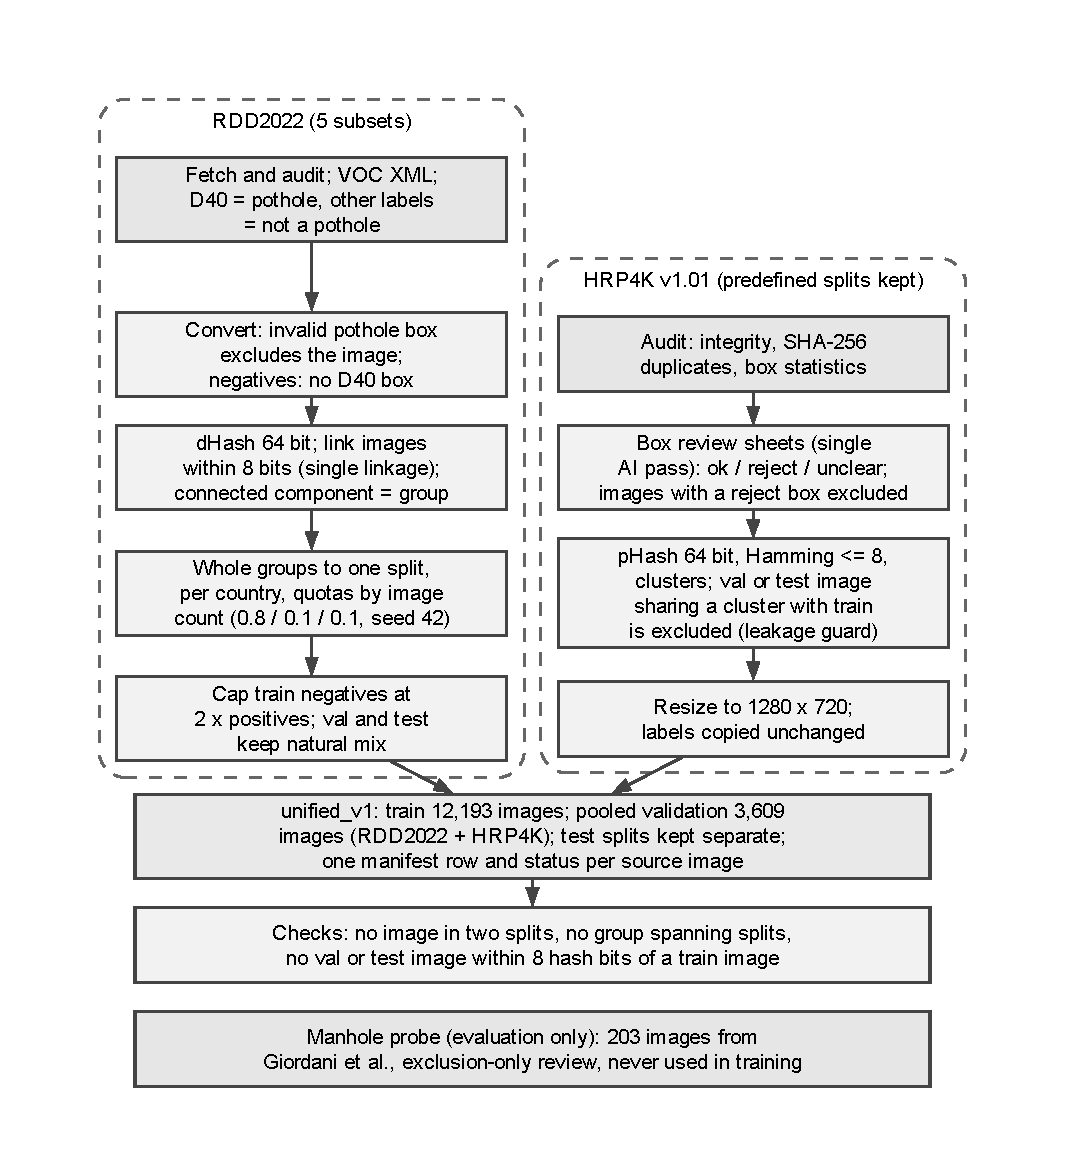
\includegraphics[width=0.68\textwidth]{ch4_datasetpipe.pdf}
\caption{Design of the dataset preparation pipeline.}
\label{fig:ch4-datasetpipe}
\end{figure}

In RDD2022 only the label D40 is a pothole; an image is positive if it has at least one D40 box and negative otherwise. Images are grouped by a 64-bit perceptual hash \cite{zauner2011rihamark}: two images of the same country are linked when their hashes differ in at most 8 bits, the connected components are the groups, and whole groups are assigned to the training, validation and test splits (80/10/10, seed 42). Grouping replaced an earlier split by blocks of image identifiers, which leaked because the identifiers are not in capture order. HRP4K keeps its predefined split, and a leakage guard removes any validation or test image that shares a hash cluster with a training image. Label review follows an exclusion-only rule: images may be removed, but boxes are never edited, added or relabelled. The same groups serve as the resampling units of the bootstrap (Section~\ref{sec:ch6-protocol}).

\section{Detector Architecture}\label{sec:ch4-yolo}
The detector is YOLOv8s \cite{jocher2023yolov8}, a single-stage detector of the YOLO family \cite{redmon2016yolo}, with one output class and 11,135,987 parameters. Figure~\ref{fig:ch4-yolov8s} shows its structure as defined in Ultralytics 8.4.210. The backbone downsamples the image to strides 8, 16 and 32 using C2f blocks, which build on the cross-stage partial idea \cite{wang2020cspnet}, and ends with a fast spatial pyramid pooling block. The neck fuses the three scales along top-down and bottom-up paths \cite{lin2017fpn,liu2018panet}, giving $80\times80$, $40\times40$ and $20\times20$ output maps at 640 px. The anchor-free head predicts boxes as distributions over the distances to the four sides \cite{li2020generalized} and one class logit per location, and training assigns positives with a task-aligned assigner \cite{feng2021tood}. Training starts from COCO-pretrained weights \cite{lin2014coco}.

\begin{figure}[!htbp]
\centering
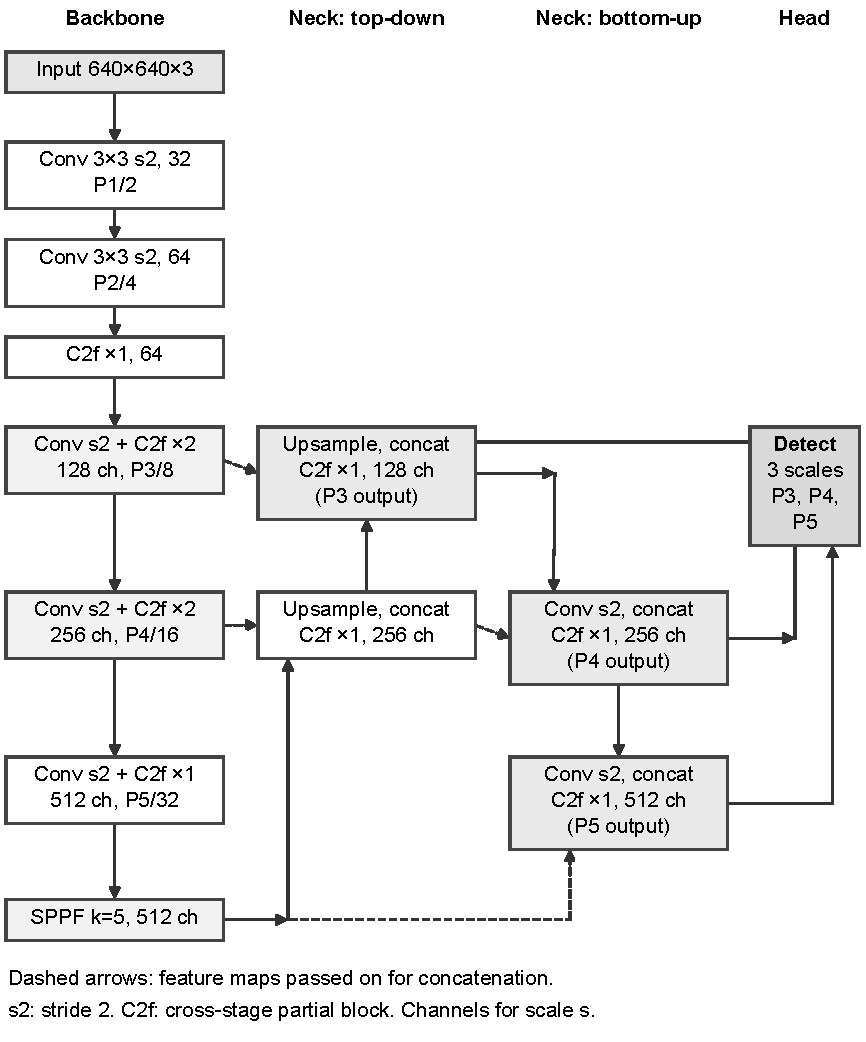
\includegraphics[width=0.62\textwidth]{ch4_yolov8s.pdf}
\caption{Structure of YOLOv8s with one class, drawn from the Ultralytics 8.4.210 model definition.}
\label{fig:ch4-yolov8s}
\end{figure}
